% HCLT 2025 — 논문 스켈레톤 (틀)
% 컴파일: pdflatex main -> bibtex main -> pdflatex main x2
% 각 절 맨 앞 %[계획] 주석 = 무슨 내용/어떤 실험(step)/어떤 주장/어떤 그림을 넣을지.
\documentclass[twocolumn, 10pt]{article}
\usepackage{hclt}
\usepackage[utf8]{inputenc}
\usepackage[pdfencoding=auto]{hyperref}
\usepackage{url}
\usepackage{amsmath}
\usepackage{latexsym}
\usepackage{amssymb}
\usepackage{graphicx}

\DeclareMathOperator*{\argmax}{arg\,max}

% 제목은 한 줄에 들어오게(길면 5.5cm 제목상자를 넘겨 아래와 겹침). 최종 제목은 연구자가 정함.
\title[korean]{표기 규약 실패는 어텐션이 아니라 후반층 값의 문제다}
\title[english]{Naming-Convention Failures: A Late-Layer Value Problem}

% 주의: hclt.sty의 \author는 인자 3개로 정의돼 있어(템플릿), 뒤에 빈 {}를 하나 더 붙인다.
\author[korean]{익명 저자$^{\circ}$ \\ 소속 \\ \texttt{email@domain}}{}
\author[english]{Anonymous \\ Affiliation}{}

% \finalcopy % 최종본에서 주석 해제

\begin{document}

\twocolumn[
\maketitle
\begin{abstract}
%[계획] 5~6문장: 문제(표기 규약 지침 위반) → 기존 관점(어텐션을 덜 본다, Spotlight) →
%       우리 방법(관측+인과 개입, 4모델, 전 층 스윕) → 발견(코드·지침 모두 후반층 Value가
%       원인, 어텐션 아님) → 처방(그 층 Value 조향이 어텐션 증폭보다 낫다).
코드 생성 언어모델은 함수 이름의 표기 규약(camelCase/snake\_case) 지침을 자주 어긴다.
기존 접근은 이를 \emph{지침을 덜 본다}는 문제로 보고 지침 토큰의 어텐션을 키운다.
본 연구는 관측과 인과 개입을 4개 모델에 적용해, (1) 모델은 지침 지시어를 충분히 보며,
(2) 코드 문맥 신호와 지침의 영향력이 모두 \emph{어텐션이 아니라 후반부 특정 층의
값(Value)}에 있음을 보인다. 값만 바꾸면 행동이 되돌아오거나 넘어가지만 어텐션만 바꾸면
그렇지 않다. 이로부터 어텐션을 키우는 접근이 겨눈 부품이 틀렸음을 주장하고, 해당 층의
값을 직접 조향하는 처방이 어텐션 증폭보다 낫다는 것을 보인다.
\end{abstract}

\begin{keyword}
코드 언어모델, 기계적 해석가능성, 활성 조향, 표기 규약, 지시 이행
\end{keyword}
]

% =====================================================================
\section{서론}
%[계획][주장] 병목은 어텐션이 아니라 후반층 Value. [그림1=티저: 절벽 or 요약]
%  - 문제제기: 코드 LLM이 표기 규약 지침을 자주 어김(예시 1개).
%  - 기존 관점/처방: 어텐션을 키운다(Spotlight~\cite). 가정: "지침을 덜 본다".
%  - 우리 반박의 씨앗: 지침은 충분히 읽힌다(step4). 그런데도 어긴다 → 문제는 "본 내용".
%  - 기여 3가지(아래 enumerate).
코드 생성 모델에게 ``함수 이름을 camelCase로 쓰라''고 지시해도, 문맥에 다른 표기가
섞이면 모델은 지침을 어기고 문맥을 따라간다. 기존 연구는 이를 모델이 지침을 충분히
주목(attention)하지 못한 탓으로 보고, 지침 토큰의 어텐션을 동적으로 키우는
방법을 제안했다~\cite{venkateswaran:spotlight, zhang:pasta}.

본 연구는 이 진단이 틀렸음을 주장한다. 관측과 인과 개입을 통해, 모델은 지침 지시어를
이미 충분히 보고 있으며(따라서 미주목은 원인이 아니며), 실패의 원인과 해결의 손잡이가
모두 \emph{모델 후반부 특정 층이 실어 나르는 값(Value)}에 있음을 보인다.

본 논문의 기여는 다음과 같다.
\begin{enumerate}
  \item 코드 문맥 신호와 지침의 영향력을 \emph{인과 개입}으로 후반층 Value에 국소화한다.
  \item 어텐션을 키우는 접근이 겨눈 지점이 원인이 아님을 4개 모델에서 일관되게 보인다.
  \item 국소화한 층의 Value를 직접 조향하는 처방이 어텐션 증폭보다 준수율을 더 올림을 보인다.
\end{enumerate}

% =====================================================================
\section{관련 연구}
%[계획] 문단 2~3개로 압축.
%  (1) 어텐션 조향: Spotlight~\cite{venkateswaran:spotlight}, PASTA~\cite{zhang:pasta}.
%  (2) 활성/표현 조향(우리 처방 계열): CAA~\cite{rimsky:caa}, ITI~\cite{li:iti},
%      Function Vectors~\cite{todd:functionvectors}.
%  (3) 기제 해석·인과 추적: ROME~\cite{meng:rome}, 트랜스포머~\cite{vaswani:attention}.
지침 이행을 개선하려는 접근은 크게 두 갈래다. 하나는 지침 토큰의 \emph{어텐션}을
사후 조정하는 방법이고~\cite{venkateswaran:spotlight, zhang:pasta}, 다른 하나는
잔차 스트림의 \emph{활성(값)}을 대조쌍으로 조향하는
방법이다~\cite{rimsky:caa, li:iti, todd:functionvectors}.
본 연구는 인과 추적~\cite{meng:rome} 기법으로 표기 규약 신호가 어느 통로·어느 층에
있는지를 특정하고, 그 결과가 후자(값 조향)를 지지함을 보인다.

% =====================================================================
\section{실험 설정}
%[계획] 데이터·모델·지표·방법. [표1=실험↔RQ 매핑]
\subsection{데이터셋과 모델}
%  - 함수 이름 504개(동사50×명사50, 겹침 없이), 12개씩 42묶음(풀 전체 커버).
%  - 함수 본문 동일(값 반환), 표기만 변수 → 통제.
%  - 모델 4개: Qwen2.5-Coder-3B~\cite{qwen:coder}, DeepSeek-Coder-6.7B~\cite{deepseek:coder},
%    Llama-3.2-3B~\cite{llama:3}(범용 대조), StableCode-3B. 시드 42 고정.

\subsection{측정과 개입}
%  - 준수 선호 S = logP(준수 이름) - logP(위반 이름) (생성 안 하고 후보 채점).
%  - 준수율: 실제 생성한 첫 함수 이름의 표기(step1).
%  - 되돌림(RQ2)/넘어감(RQ3) = (S_개입 - S_base)/(S_기준 - S_base).
%  - 개입: 대상 토큰의 KV를 반대 조건 것으로 평균 덮어쓰기(mean-pool),
%    어텐션만(Key)/내용만(Value)/둘다, 전 층 스윕.
%  - 판정불가: 기준-base 차<1.0(레버 없음)이면 제외.

\begin{table}[t]
\caption{실험 구성과 연구질문 매핑}
\label{tab:exp}
\begin{center}
\small
\begin{tabular}{c|l|c|c}
\hline
스텝 & 무엇을 보나 & RQ & 유형 \\
\hline
step1 & 준수율 절벽 & RQ1 & 생성 \\
step2 & 코드 신호 관측 & RQ2 & 관측 \\
step3 & 코드 신호 인과 & RQ2 & 개입 \\
step4 & 지침 지시어 관측 & RQ3 & 관측 \\
step5 & 지침 지시어 인과 & RQ3 & 개입 \\
step6 & 값 조향 처방 & --- & 처방 \\
\hline
\end{tabular}
\end{center}
\end{table}

% =====================================================================
\section{결과}

\subsection{RQ1: 표기 규약 실패는 실재한다}
%[계획][step1][주장] 문맥 위반↑ → 준수율 급락(절벽). 양방향(camel/snake).
%  [그림: 절벽 곡선 — step1 결과 나오면 삽입. 지금은 자리만.]
%  - 위반 개수 0~12 스윕 × 지침 방향 2종(파이썬).
%  - 결론: 실패가 있다 → "왜?"로 넘어감(RQ2, RQ3).
\emph{[step1 결과 삽입 예정: 위반 개수 대 준수율 절벽 곡선.]}

\subsection{RQ2: 코드 신호는 어텐션이 아니라 후반층 값이다}
%[계획][step2 관측 + step3 인과][주장] 코드 표기 신호 = Value, 후반 단일 층.
%  관측(step2): ‖v‖는 camel/snake 동일, av 격차는 후반층 → 관측만으론 분리 불가.
%  인과(step3): 위반 이름 KV를 준수판으로 치환 → Value 되돌림 > Key,
%    후반 봉우리 층, 형태 전이(다른 camel도 됨), 표기 특정(다른 snake는 안 됨=음성통제).
%  [그림2=step3 되돌림(Value vs Key), 그림3=공여 통제]
관측 단계에서 두 표기의 값 크기(\(\|v\|\))는 사실상 동일하고 차이는 후반층의
기여량에 나타나, 관측만으로는 어텐션과 값을 가를 수 없다(그림~\ref{fig:rq2av}).
인과 개입에서, 문맥 위반 이름의 값을 준수판으로 바꾸면 준수 선호가 특정 후반 층에서
되돌아오는 반면 어텐션만 바꾸면 그렇지 않다(그림~\ref{fig:rq2rec}). 되돌림은
\emph{형태 전이}(무관한 camel 이름으로도 동일)와 \emph{표기 특정성}(무관한 snake로는
되돌지 않음, 음성통제)을 보여, 트리비얼한 효과가 아님을 확인한다(그림~\ref{fig:rq2donor}).

\begin{figure}[t]
\centering
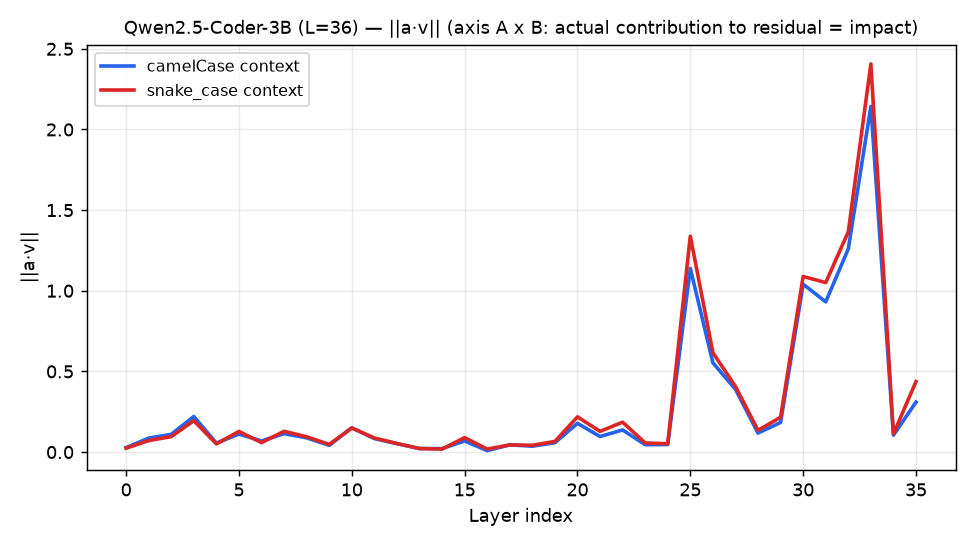
\includegraphics[width=.46\textwidth]{figures/rq2_av_qwen.png}
\caption{RQ2 관측(step2): 두 표기의 기여량 격차는 후반층에 나타난다(Qwen).}
\label{fig:rq2av}
\end{figure}

\begin{figure}[t]
\centering
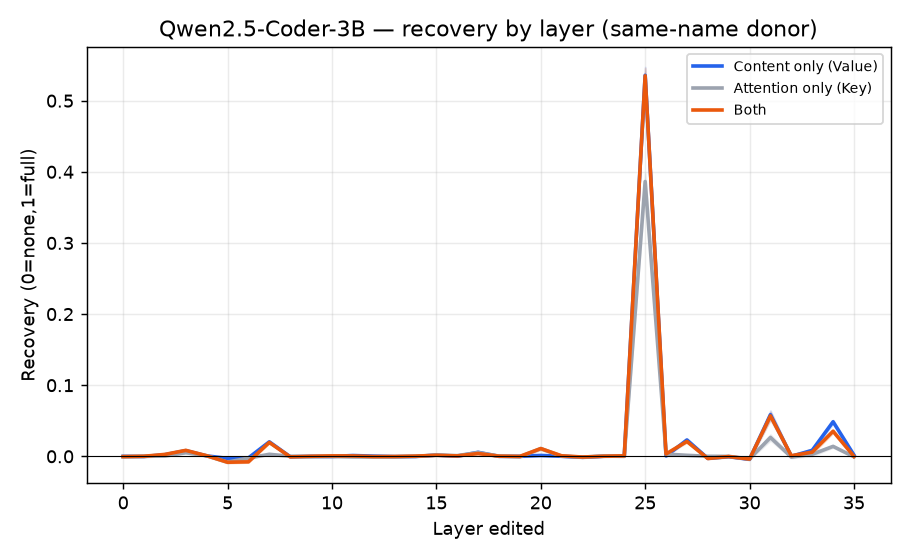
\includegraphics[width=.46\textwidth]{figures/rq2_recovery_qwen.png}
\caption{RQ2 인과(step3): 내용(Value)만 후반 층에서 준수를 되돌린다. 어텐션(Key)만은 약하다(Qwen, 95\% 신뢰구간).}
\label{fig:rq2rec}
\end{figure}

\begin{figure}[t]
\centering
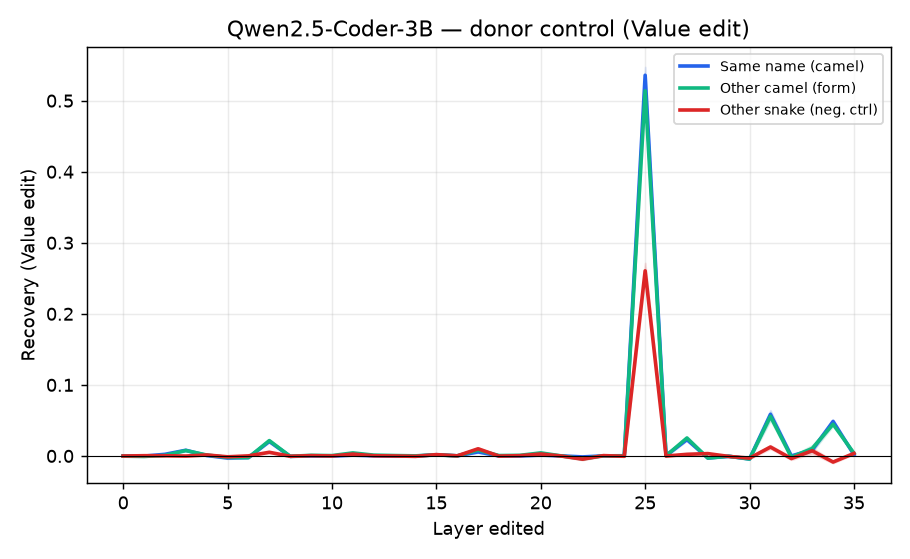
\includegraphics[width=.46\textwidth]{figures/rq2_donor_qwen.png}
\caption{RQ2 통제(step3): 같은 camel$\approx$다른 camel(형태 전이), 다른 snake는 낮음(음성통제).}
\label{fig:rq2donor}
\end{figure}

\subsection{RQ3: 지침도 같은 통로·같은 층이다}
%[계획][step4 관측 + step5 인과][주장] 지침도 Value, 코드와 같은 후반층.
%  관측(step4): 토큰당 어텐션에서 지시어를 코드 이름만큼(또는 더) 본다 → 미주목 반박.
%  인과(step5): 지시어 Value를 반대 지침 것으로 치환 → 넘어감 Value≫Key,
%    봉우리 층이 step3 코드 층과 1~3층 차이로 겹침 → "층 어긋남" 가설 반박.
%  범용 모델(llama)은 지침 레버 약해 판정불가 → RQ3는 코드전용 3모델 한정(한계로 명시).
%  [그림4=step4 어텐션 요약, 그림5=step5 넘어감+층비교, 표2=4모델 종합]
모델은 지침 지시어를 코드 이름만큼(또는 그 이상) 본다(그림~\ref{fig:rq3attn}). 따라서
미주목은 원인이 아니다. 인과 개입에서 지시어의 값을 반대 지침 것으로 바꾸면 행동이
반대 지침으로 넘어가며, 이 역시 어텐션이 아니라 값이 주도한다(그림~\ref{fig:rq3trans}).
넘어감의 봉우리 층은 코드의 인과 층(step3)과 1$\sim$3층 차이로 겹쳐, 두 신호가 같은
후반 층에서 작동함을 보인다(표~\ref{tab:peak}). 다만 범용 모델은 지침의 영향력 자체가
약해 판정불가로 분류한다(§\ref{sec:limit}).

\begin{figure}[t]
\centering
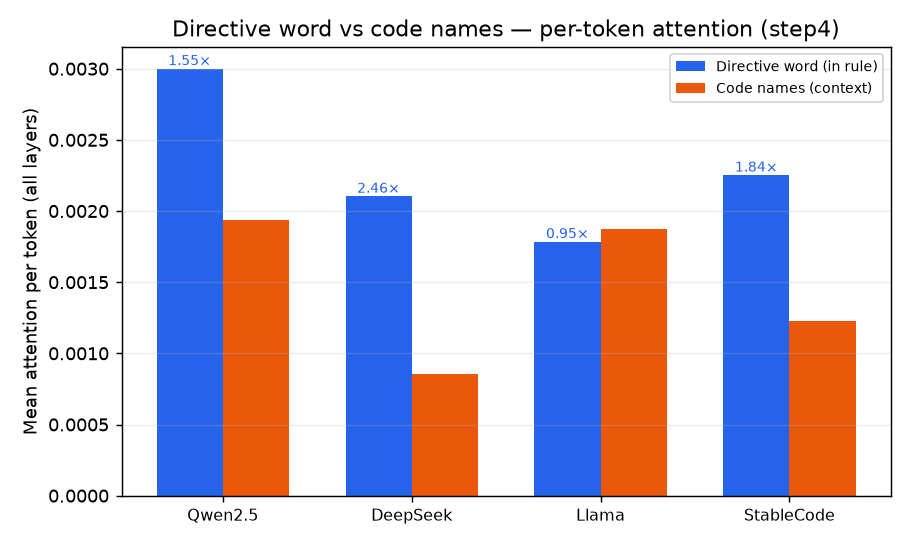
\includegraphics[width=.46\textwidth]{figures/rq3_attention_summary.png}
\caption{RQ3 관측(step4): 토큰당 어텐션에서 지시어를 코드 이름만큼 본다.}
\label{fig:rq3attn}
\end{figure}

\begin{figure}[t]
\centering
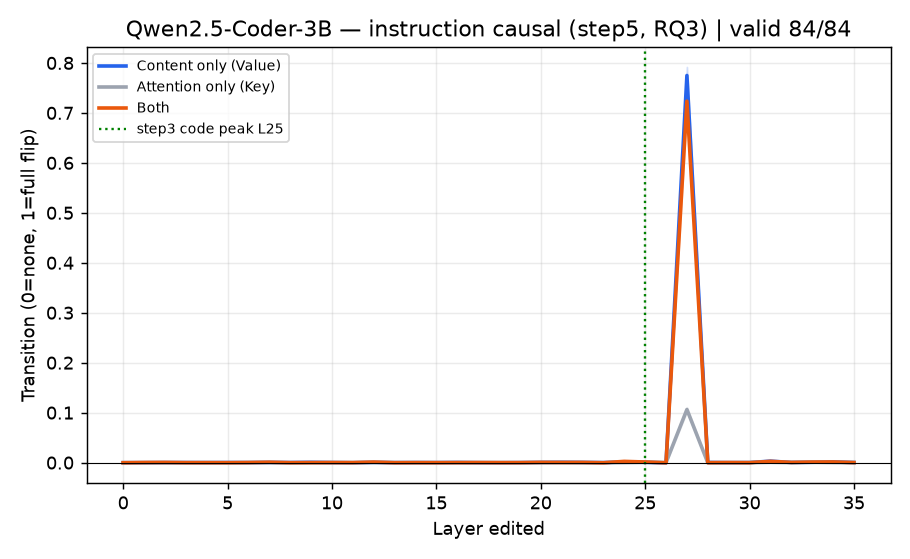
\includegraphics[width=.46\textwidth]{figures/rq3_transition_qwen.png}
\caption{RQ3 인과(step5): 지시어 값(Value)만 행동을 반대 지침으로 넘긴다. 초록 점선=코드 인과 층(step3).}
\label{fig:rq3trans}
\end{figure}

\begin{table}[t]
\caption{모델별 인과 봉우리 층과 값$-$어텐션 격차(±95\% 신뢰구간). llama는 판정불가.}
\label{tab:peak}
\begin{center}
\small
\begin{tabular}{l|c|c|c}
\hline
모델 & 코드층 & 지침층 & 값$-$어텐션(지침) \\
\hline
Qwen-3B     & 25 & 27 & $+$0.67 \\
DeepSeek-6.7B & 20 & 17 & $+$0.24 \\
StableCode-3B & 18 & 19 & $+$0.66 \\
Llama-3.2-3B & 15 & --- & 판정불가 \\
\hline
\end{tabular}
\end{center}
\end{table}

% =====================================================================
\section{처방: 값 조향이 어텐션 증폭보다 낫다}
%[계획][step6][주장] 국소화한 후반층 Value에 대조 조향 벡터(CAA~\cite{rimsky:caa})를
%  더해 준수율↑. 어텐션 증폭(Spotlight/PASTA)보다 낫고, 잘못된 층엔 안 됨(통제).
%  [그림6=CAA vs Spotlight 준수율, α 용량-반응 곡선]
앞서 특정한 후반 층의 값에, 대조쌍(camel$-$snake)에서 얻은 조향 벡터를
더한다~\cite{rimsky:caa}. 이는 어텐션을 키우는 접근과 달리 원인 부품을 직접 겨냥한다.
\emph{[step6 결과 삽입 예정: 준수율의 용량-반응 곡선, Spotlight/PASTA 대비, 잘못된 층 통제.]}

% =====================================================================
\section{논의 및 한계}
\label{sec:limit}
%[계획]
%  - 좁음: 규약 1종(camel/snake), 인공 함수 이름, 파이썬 위주.
%  - 범용 모델(llama)은 지침 레버 약해 판정불가 → 결론은 코드전용 3모델 한정.
%  - 되돌림/넘어감이 부분적(한 층만 고쳐선 완전 회복 아님).
%  - 어텐션도 완전 0은 아님: 주장은 "값 우위·값 충분"이지 "어텐션 무관"이 아님.

% =====================================================================
\section{결론}
%[계획] 한 문단: 표기 규약 실패의 자리는 후반층 Value이며 어텐션이 아니다.
%  따라서 처방은 그 값을 고치는 것. 코드·지침이 같은 통로·같은 층.

\bibliographystyle{IEEEtran}
\bibliography{refer}

\end{document}
